\documentclass{beamer}

\usepackage[progressbar=foot]{theme/beamerthememetropolis}           % Use metropolis theme
\usepackage{my-commands}
\usepackage{amsmath}
\usepackage{marvosym}

\title{\godels{} Incompleteness Theorems}

\date{\today}
\author{Scott Sanderson (@scottbsanderson)}
\institute{Papers We Love - Boston}

\begin{document}
\maketitle

\section{The Stage}

\begin{frame}{Hilbert's Program}
  \begin{columns}
    \column{0.5\textwidth}
    \begin{block}{David Hilbert}
      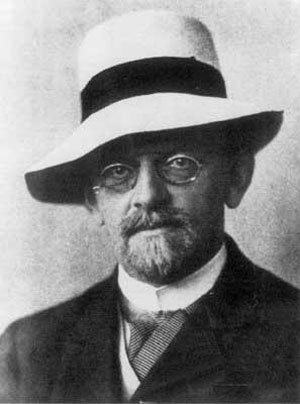
\includegraphics[width=0.75\textwidth]{images/hilbert.jpg}
    \end{block}

    \column{0.5\textwidth}
    \begin{itemize}
    \item[]<1-> In 1900, published a list of the 23 most important unsolved
      problems in mathematics for the 20th century.
    \item[]<2-> Problem 2 is ``prove the consistency of aritmetic''.
    \end{itemize}

  \end{columns}
\end{frame}

\begin{frame}{Principia Mathematica and Russell's Logicism}
  \begin{columns}[c]

    \column{0.5\textwidth}
    \begin{block}{Alfred North Whitehead}
      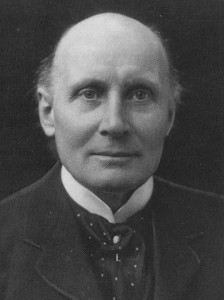
\includegraphics[height=0.35\textheight]{images/whitehead.jpg}
    \end{block}

    \begin{block}{Bertrand Russell}
      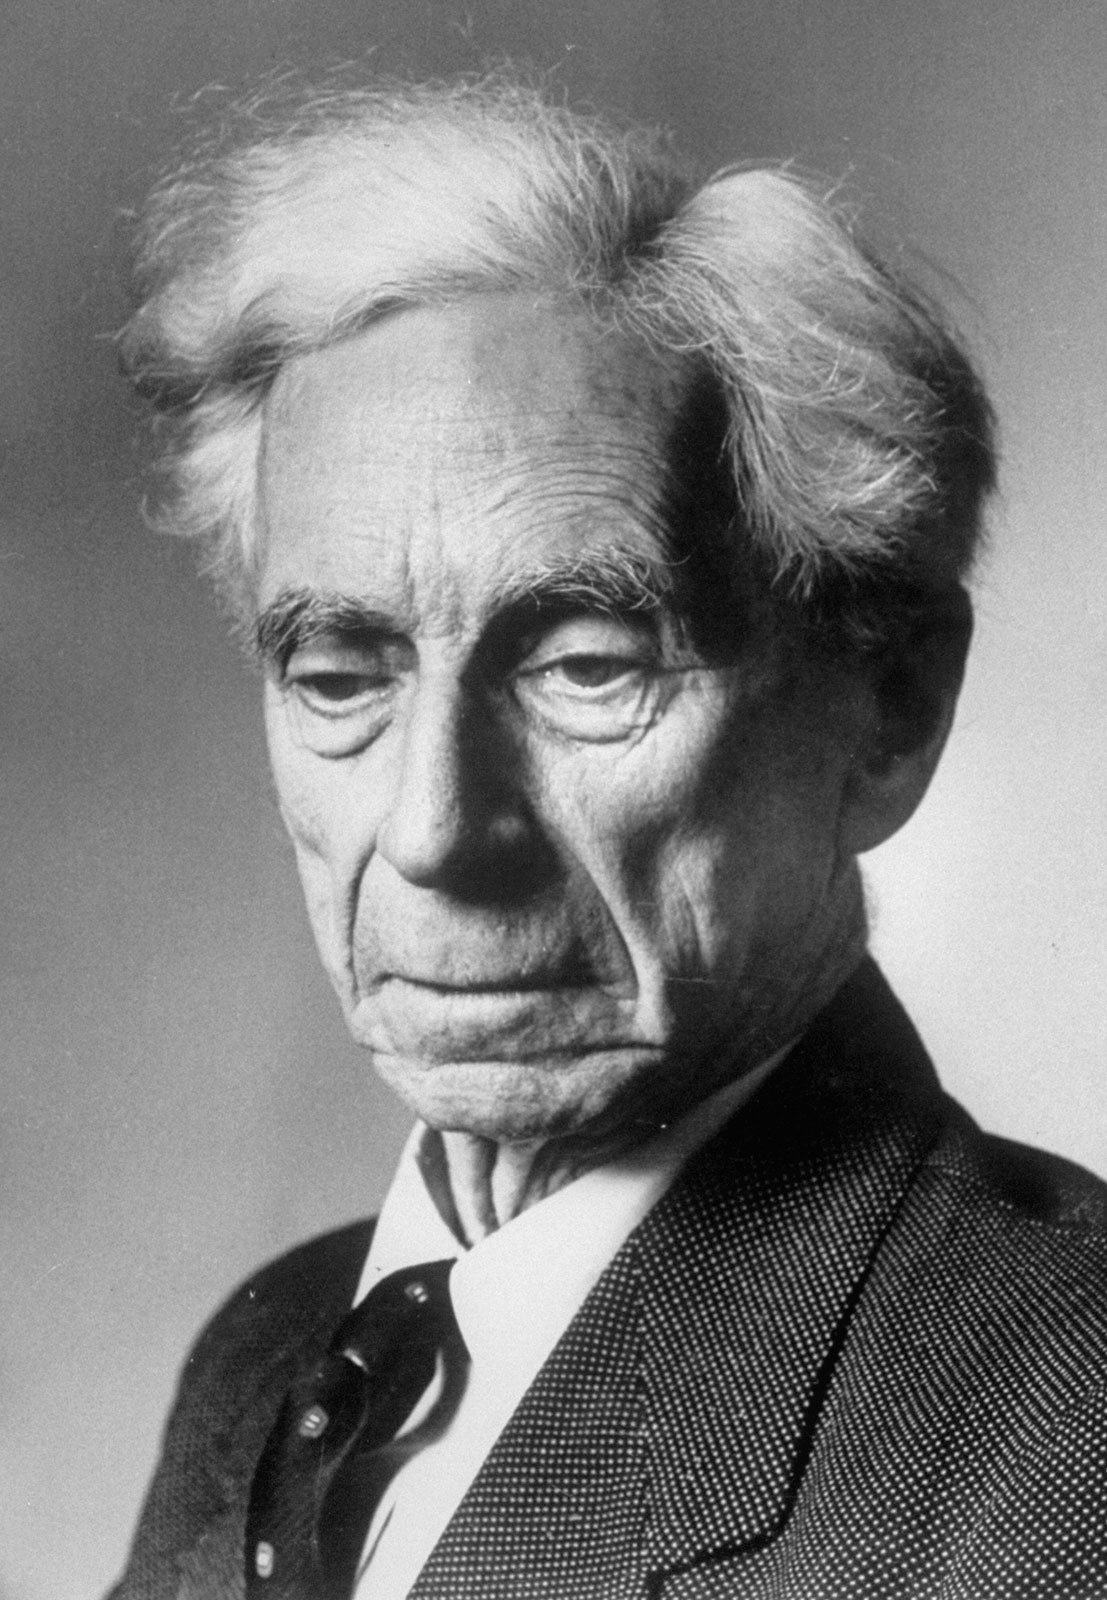
\includegraphics[height=0.35\textheight]{images/russell.jpg}
    \end{block}

    \column{0.5\textwidth}
    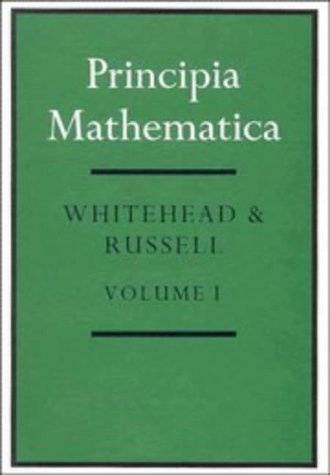
\includegraphics[height=0.75\textheight]{images/principia.jpg}

  \end{columns}
\end{frame}

\section{The Paper}

\begin{frame}{The Paper}
  \begin{columns}

    \column{0.5\textwidth}
    \begin{figure}
      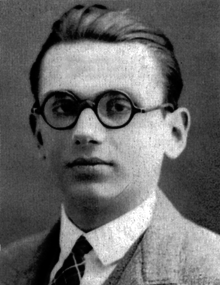
\includegraphics[scale=0.45]{images/godel.png}
    \end{figure}

    \column{0.5\textwidth}
    \begin{figure}
      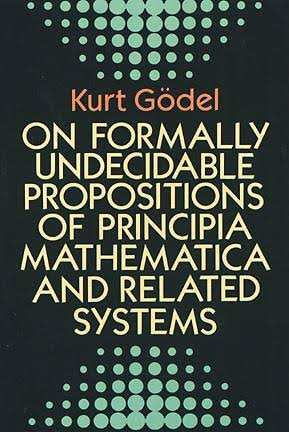
\includegraphics[scale=0.45]{images/godel-book.jpg}
    \end{figure}

  \end{columns}
\end{frame}

\begin{frame}{Informal Statement of the Incompleteness Theorems}
  \begin{theorem}[\godels{} First Incompleteness Theorem]
    Let $F$ be a consistent formal system that can express arithmetic. There
    are statements well-formed statements in the language of $F$ which are
    neither provable nor disprovable in $F$.
  \end{theorem}

  \pause

  \begin{theorem}[\godels{} Informal Statement of the Second Incompleteness Theorem]
    Let $F$ be a consistent formal system that can express arithmetic. $F$
    cannot prove its own consistency.
  \end{theorem}
\end{frame}

\begin{frame}{lolwut?}
  What do we mean by ``formal system''?

  \pause

  What does it mean for $F$ to be ``consistent''?

  \pause

  How can a statement be neither provable nor disprovable?

  \pause

  What would it mean for $F$ to prove its own consistency?
\end{frame}

\begin{frame}{What is a Formal System?}

  A \textbf{formal system} $F$ is:
  \begin{itemize}
  \item An \textbf{alphabet} of symbols (e.g. $0, ', \neg, \exists, \forall, \rightarrow$).
  \item A \textbf{grammar}, describing the strings of symbols that are
    \textbf{well-formed} sentences.
  \item A set of \textbf{axioms} containing initial theorems of $F$.
  \item A set of \textbf{rules of inference} describing how to transform
    existing theorems into new theorems.
  \end{itemize}

\end{frame}

\begin{frame}{Robinson Arithmetic}
  \textbf{Robinson Arithmetic} (\robinson) is a simple axiomatization of
  arithmetic on the natural numbers.

  \pause

  Defines $+$ and $\times$ in terms of \textbf{successor} $'$.

  \pause

  $0$ is the only constant. Other numeric constants written as $0'''...'$.

\end{frame}

\begin{frame}{Robinson Arithmetic}
  \begin{block}{Symbols}
    \begin{itemize}
    \item[] $0, ', \neg, =, +, \times, \land, \lor, \forall, \exists, \rightarrow, (, )$
    \item[] $a, b, c, \dots, x, y, z, \dots$ (as many as needed)
    \end{itemize}
  \end{block}
\end{frame}

\begin{frame}{Robinson Arithmetic}
  \begin{block}{Well-Formed Sentences}
    \begin{itemize}
    \item[] $0 + 0 = 0$
    \item[] $0' + 0' = 0''$
    \item[] $\forall x(x + 0 = x)$
    \item[] $\forall x \exists y(y + y = x)$
    \end{itemize}
  \end{block}
  \begin{block}{Invalid Sentences}
    \begin{itemize}
    \item[] $'0$
    \item[] $= +xy$
    \item[] $\forall \exists$
    \end{itemize}
  \end{block}
\end{frame}

\begin{frame}{Robinson Arithmetic}
  \begin{block}{Axioms}
    \begin{enumerate}
    \item<1-> $\forall x (\neg (0 = x'))$
    \item<2-> $\forall x \forall y (x' = y' \rightarrow x = y)$
    \item<3-> $\forall x (\neg (x = 0) \rightarrow \exists y (x = y'))$
    \item<4-> $\forall x (x + 0 = 0)$
    \item<5-> $\forall x ((x + y') = (x + y)')$
    \item<6-> $\forall x (x \times 0 = 0)$
    \item<7-> $\forall x \forall y (x \times y' = (x \times y) + x)$
    \end{enumerate}
  \end{block}
\end{frame}

\begin{frame}{Robinson Arithmetic}
  \begin{block}{Rules of Inference}
    \begin{itemize}
    \item[] $p, (p \rightarrow q) \vdash q$
    \item[] $\neg \neg p \rightarrow p$
    \item[] $p \land q \vdash p$
    \item[] $(p \rightarrow q) \vdash (\neg q \rightarrow \neg p)$
    \item[] $\dots$
    \end{itemize}
  \end{block}
\end{frame}

\begin{frame}{Consistency}

  A formal system $F$ is \textbf{inconsistent} if, for some proposition $p$:

  $$F \vdash p$$
  and
  $$F \vdash \neg p$$

  \pause

  A formal system is \textbf{consistent} if it is not inconsistent.

\end{frame}

\section{The First Theorem}

\begin{frame}{The First Incompleteness Theorem}
  \begin{theorem}[First Incompleteness Theorem]
    Let $F$ be a consistent formal system that contains \robinson{}. Then we
    can construct a sentence $G_F$ such that:

    \begin{enumerate}
    \item $F \nvdash G_F$.
    \item $F \nvdash \neg G_F$.
    \end{enumerate}

  \end{theorem}
\end{frame}

\begin{frame}{Liar Paradox}
  Consider the sentence \textbf{``This sentence is false.''}.

  \pause

  \begin{itemize}
  \item[] If it's true, then by its own assertion it must be false. \Frowny
    \pause
  \item[] If it's false, then, by its own assertion, it must be true. \Frowny
  \end{itemize}

  \pause

  Many answers have been proposed for how to understand the logical content of
  this sentence.

\end{frame}

\begin{frame}{Proof Paradox}

  Consider the sentence \textbf{``This sentence is not provable''}.

  \pause

  \begin{itemize}
  \item[] If it's provable, then we have a proof that the sentence isn't
    provable. \Frowny \pause
  \item[] If it's not provable, then we don't have such a proof. \Smiley
    \pause
  \end{itemize}

  If our deductive system is consistent, then the sentence is true, which means
  we can't prove that it's true

\end{frame}

\begin{frame}{Proof Idea for First Incompleteness Theorem}

  \begin{block}{Proof Idea}
    Construct a sentence in \robinson{} that asserts its own unprovability.
  \end{block}

\end{frame}

\begin{frame}{Representability}
  \begin{definition}[Weak Representability]
    A set $S$ of natural numbers is \textbf{weakly representable} in $F$ if
    there exists a formula $A(x)$ in the language of $F$ such that:

    $$n \in S \iff F \vdash A(\underline{n}) $$
  \end{definition}
\end{frame}

\begin{frame}{Representability}
  \begin{definition}[Strong Representability]
    A set $S$ of natural numbers is \textbf{strongly representable} in $F$ if
    there exists a formula $A(x)$ in the language of $F$ such that:

    $$n \in S \implies F \vdash A(\underline{n})$$
    $$n \notin S  \implies F \vdash \neg A(\underline{n})$$

  \end{definition}
\end{frame}

\begin{frame}{Representability (in plain English)}
  Weak representability means that we can write down a formula $A$ such that
  $F$ proves $A(\underline{x})$ whenever $x \in S$.

  \pause

  Strong representability means that can write down a formula $A$ such that $F$
  proves $A(\underline{x})$ whenever $x \in S$ \textbf{and} $F$ proves
  $\neg A(\underline{x})$ whenever $x \notin S$.

  \pause

  We can define representability for relations analogously using formulae with
  more than one free variable.
\end{frame}

\begin{frame}{Examples of Representability}

  \begin{align*}
    Even(x) & \equiv \exists y (x = y \times 0'') \\
    Odd(x) & \equiv \exists y(x = y' \land Even(y)) \\
    LessThan(x, y) & \equiv \exists n (x + n' = y) \\
    Divides(x, y) & \equiv \exists n (n \times y = x) \\
    Prime(x) & \equiv \forall y((Divides(x, y) \rightarrow (y = 0' \lor y = x)))
  \end{align*}

\end{frame}

\begin{frame}{\godel{} Numbering}
  \begin{block}{Problem}
    How to make assertions about provability of \robinson{}-sentences in
    \robinson{}?
  \end{block}

  \pause

  \begin{block}{Idea}
    Encode assertions about proofs as assertions about numbers.
  \end{block}

  \pause

  Requires that we can produce a correspondence between numbers and sentences.

\end{frame}

\begin{frame}{\godel{} Numbering}
  Assign a positive integer to each symbol in the alphabet of the
  language of $F$.

  \begin{columns}[T]
    \column{0.25\textwidth}
    $$C(0) = 1$$
    $$C(') = 2$$
    $$C(+) = 3$$
    $$C(\times) = 4$$

    \column{0.25\textwidth}

    $$C(=) = 5$$
    $$C(() = 6$$
    $$C()) = 7$$
    $$C(\rightarrow) = 8$$

    \column{0.25\textwidth}

    $$C(\neg) = 9$$
    $$C(\forall) = 10$$
    $$C(\land) = 11$$
    $$C(\lor) = 12$$

    \column{0.25\textwidth}

    $$C(a) = 13$$
    $$C(b) = 14$$
    $$\dots$$
    $$C(x_i) = 12 + i$$

  \end{columns}

\end{frame}

\begin{frame}{\godel{} Numbering}

  Encode sequences of symbols in the exponents of the powers of prime numbers.

  \begin{align*}
    \gnum{0 + 0 = 0} &= 2^{C(0)}3^{C(+)}5^{C{0}}7^{C(=)}11^{C(0)} \\
                     &= 2^13^35^17^511^1 \\
                     &= 4537890
  \end{align*}

  \pause

  We can use similar techniques to encode sequences of sequences.

\end{frame}

\begin{frame}{Encoding Proof}

  \begin{theorem}[Valid Proofs are Strongly Representable in $Q$]

    There is a formula of $F$, $Proof_F(x, y)$ that strongly represents the
    relation:

    $x$ is the \godel{} number of a proof of a formula with \godel{} number $y$

  \end{theorem}

\end{frame}

\begin{frame}{Encoding Provability}

  \begin{corollary}[Provability is Weakly Representable in $Q$]

    There is a formula of $F$, $Provable_F(x)$, that weakly represents the
    relation:

    $x$ is the \godel{} number of a provable sentence.

  \end{corollary}

  \pause

  $$Provable_F(x) \equiv \exists y (Proof_F(x, y)) $$

\end{frame}

\begin{frame}{Encoding Self-Reference}
  \begin{Theorem}[Diagonalization Lemma]

    Let $A(x)$ be a formula in the language of $F$ with one free variable. We
    can construct a sentence $D_A$ such that:

    $$F \vdash (D_A \leftrightarrow A(\gnum{D_A}))$$

  \end{Theorem}

  We refer to $D_A$ as the \textbf{diagonalization} of $A$.

\end{frame}

\begin{frame}{Proof of the First Incompleteness Theorem}

  \only<1-2>{
    Let $G_F$ be the diagonalization of $\neg Provable_F(x)$.
  }

  \only<2-5>{
    By the Diagonalization Lemma:
    \begin{equation}
      \label{1}
      F \vdash (G_F \leftrightarrow  \neg Provable_F(\gnum{G_F}))
    \end{equation}
  }

  \only<3-5>{
    \begin{block}{Suppose $F \vdash G_F$:}
      By weak representability of $Provable_F$:
      $$F \vdash Provable_F(\gnum{G_F})$$
      \uncover<4-5>{
        but by $(1)$,
        $$F \vdash \neg Provable_F(\gnum{G_F})$$
      }
      \uncover<5>{
        So, if $F$ is consistent, $F \nvdash G_F$.
      }
    \end{block}
  }

  \only<6-9>{
    \begin{block}{Suppose $F \vdash \neg G_F$:}
      No $n$ is the \godel{} number of a proof of $G_F$, so by strong
      representability of $Proof_F$, for every numeral $\underline{n}$:
      $$F \vdash \neg Proof_F(\underline{n}, \gnum{G_F}) $$
      \uncover<7->{
        We'd \textbf{like} to conclude that:
        \begin{align*}
          F & \vdash \neg \exists n( Proof(n, \gnum{G_F})) \\
          \therefore F & \vdash \neg Provable(\gnum{G_F})
        \end{align*}
      }

      \uncover<9> {
        but this actually requires a slightly stronger assumption
        $\omega$-consistency.
      }
    \end{block}
  }

\end{frame}

\begin{frame}{Consistency vs. $\omega$-Consistency}
  A formal theory is consistent if it is not the case that for some $A$:
  \begin{itemize}
  \item[] $F \vdash A$
  \item[] $F \vdash \neg A$
  \end{itemize}

  \pause

  A formal theory is \textbf{$\omega$-consistent} if is is not the case that
  for some $A(x)$:

  \begin{itemize}
  \item[] $F \vdash A(\underline{n})$ for every numeral $\underline{n}$.
  \item[] $F \vdash \exists n ( \neg A(n))$
  \end{itemize}

  \pause

  $\omega$-consistency is a stronger condition, and is what \godel{} used in
  his original proof.
\end{frame}

\begin{frame}{Final Statement of the First Incompleteness Theorem}

  \begin{theorem}[\godels{} First Incompleteness Theorem]
    Let $F$ be a formal system that contains \robinson{}. Then we can construct
    a sentence $G_F$ such that:

    \begin{enumerate}
    \item If $F$ is consistent, $F \nvdash G_F$.
    \item If $F$ is $\omega$-consistent, $F \nvdash \neg G_F$.
    \end{enumerate}

  \end{theorem}

\end{frame}

\begin{frame}{Review of First Incompleteness Theorem}
  \begin{block}{Summary:}
    \begin{itemize}
    \item<1-> We can encode statements \textbf{about statements} in arithmetic
      by \textbf{encoding statements as numbers}.
    \item<2-> We can express ``$x$ is a proof of $y$'' (suitably encoded) in
      arithmetic.
    \item<3-> We can express ``$x$ is provable'' as ``$\exists y$ s.t. $y$ is a
      proof of $x$''.
    \item<4-> Diagonalization transforms a predicate into a statement that is
      provable in iff its \godel{} numbers satisfies the predicate.
    \item<5-> Applying diagonalization to ``$x$ is not provable'' yields a
      statement that's provable only if it's not provable.
    \end{itemize}
  \end{block}
\end{frame}

\section{The Second Theorem}

\begin{frame}{The Second Incompleteness Theorem}
  \begin{theorem}[\godels{} Second Incompleteness Theorem]
    Let $F$ be a consistent formal system that contains Peano Arithmetic, and
    define:
    $$Cons_F \equiv \neg Provable_F(0 = 0')$$
    then
    $$F \nvdash Cons_F $$
  \end{theorem}

  \only<2>{
    In other words, if $F$ is consistent, then $F$ \textbf{can't prove that it doesn't
    prove contradictions}.
  }

\end{frame}

\begin{frame}{Proof Sketch}
  \begin{block}{Main Idea:}
    Let $G_F$ be the \godel{} sentence constructed in the proof of the first
    theorem. Prove
    $$F \vdash (Cons_F \leftrightarrow G_F)$$
    By the first theorem, if $F$ is consistent, then $F \nvdash G_F$.

    Therefore, $F \nvdash Cons_F$.

  \end{block}
\end{frame}

\begin{frame}{Proof Sketch}
  How do we show that $F$ proves the equivalence of $Cons_F$ and $G_F$?

  \pause

  Essentially, the idea is to translate the argument from theorem 1
  \textbf{into the language of $F$}.

  \pause

  We show that $F \vdash (\neg G_F \rightarrow \bot \rightarrow \neg Cons_F)$,
  which implies that $F \vdash Cons_F \rightarrow G_F$.

\end{frame}
\begin{frame}{Challenges}

  Derivation requires \textbf{L\"ob's Derivability Conditions} (or equivalent)
  to be shown for the provability predicate $Provable_F$ (abbreviated here as
  $Prov_F$):

  \begin{align}
    F & \vdash A \implies Prov_F(\gnum{A}) \\
    F & \vdash Prov_F(\gnum{A}) \rightarrow Prov_F(\gnum{Prov_F(\gnum{A})}) \\
    F & \vdash Prov_F(\gnum{A}) \land Prov_F(\gnum{A \rightarrow B}) \rightarrow Prov_F(\gnum{B})
  \end{align}

\end{frame}

\section{Epilogue}

\begin{frame}{Implications for Hilbert's Program}
  \begin{columns}[T]
    \column{0.35\textwidth}
    \begin{block}{David Hilbert}
      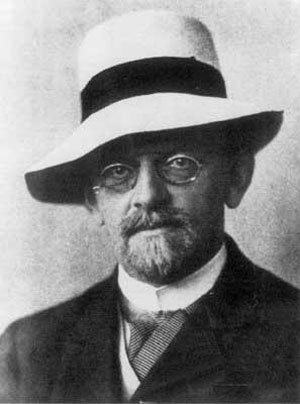
\includegraphics[width=0.75\textwidth]{images/hilbert.jpg}
    \end{block}

    \only<1-3>{
      \column{0.65\textwidth}
      \begin{itemize}
      \item[]<1-> Second Theorem rules out proving consistency of infinitistic
        mathematics using finitistic means.
      \item[]<2-> Still possible to prove arithmetic consistent via external
        means.
      \item[]<3> Proven consistent by Gentzen in 1936 using transfinite
        induction.
      \end{itemize}
    }
    \only<4>{
      \column{0.65\textwidth}
      \begin{quotation}
        It is likely that all mathematicians ultimately would have accepted
        Hilbert's approach had he been able to carry it out successfully. The
        first steps were inspiring and promising. But then G\"odel dealt it a
        terrific blow (1931), from which it has not yet recovered.

        --- Hermann Weyl (1946)
      \end{quotation}
    }
  \end{columns}

\end{frame}

\begin{frame}{Implications for Logicism}
  \begin{columns}[c]

    \column{0.5\textwidth}
    \begin{block}{Alfred North Whitehead}
      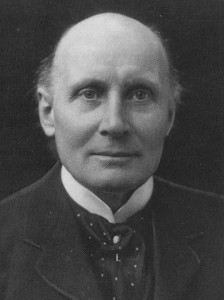
\includegraphics[height=0.35\textheight]{images/whitehead.jpg}
    \end{block}

    \begin{block}{Bertrand Russell}
      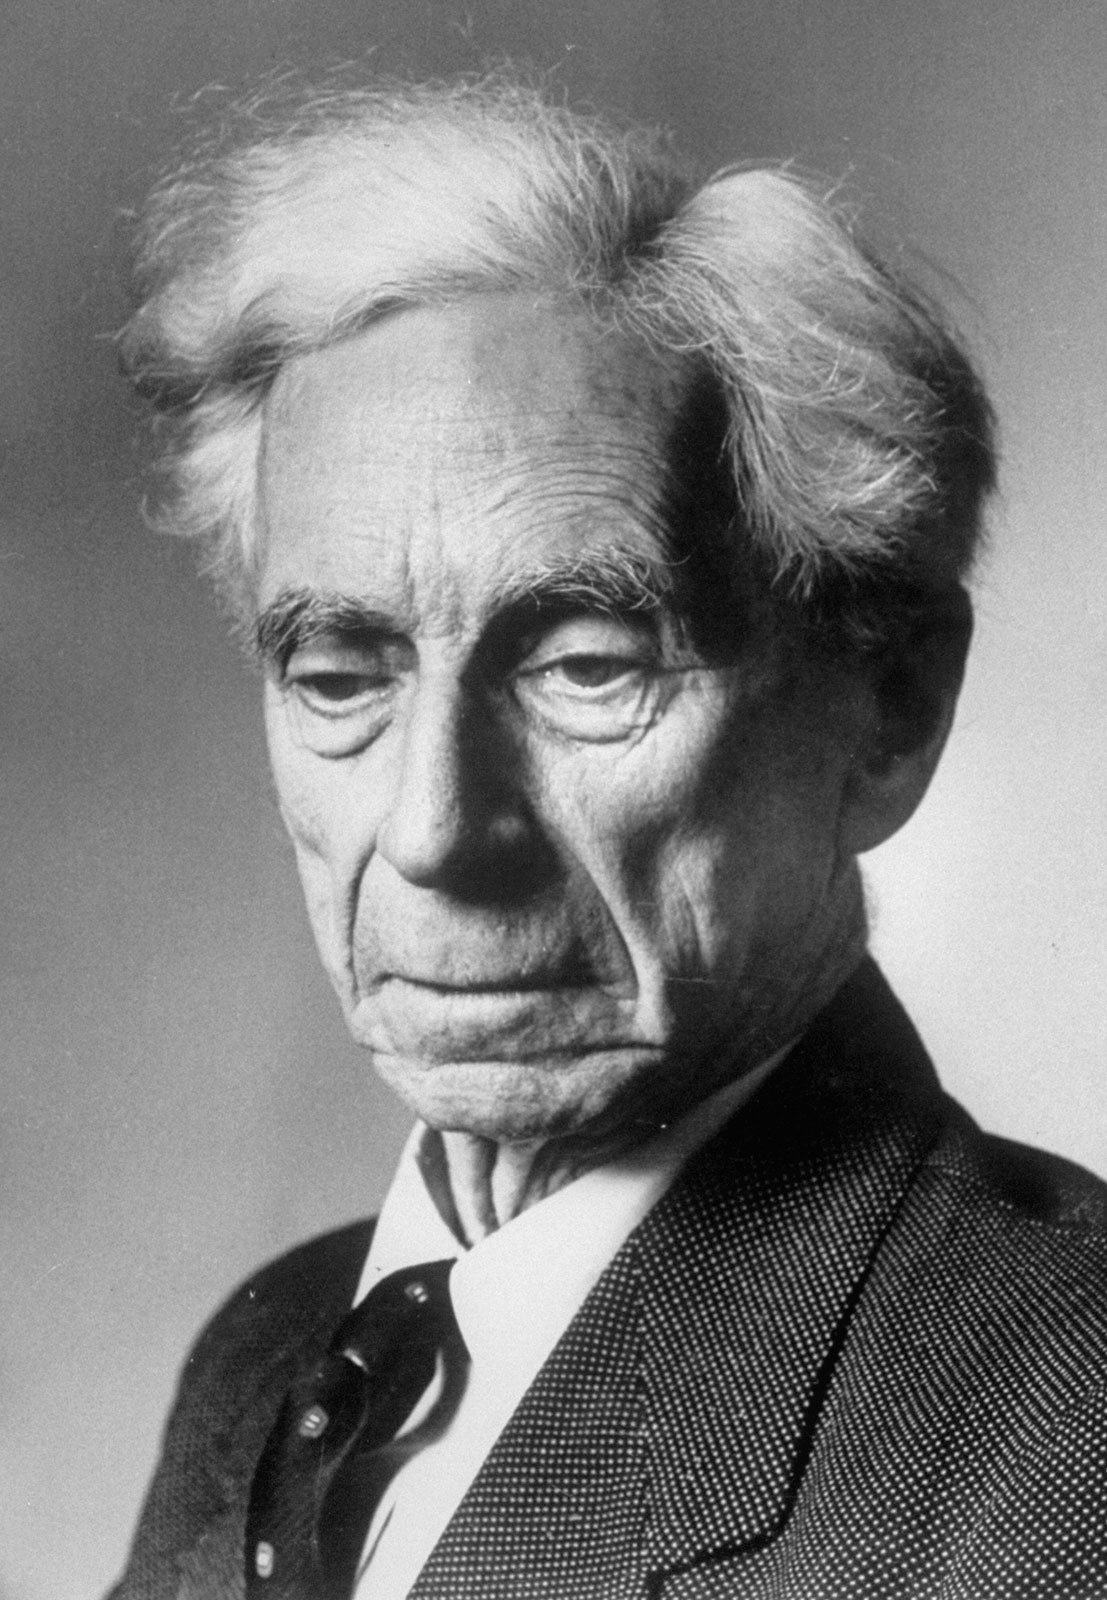
\includegraphics[height=0.35\textheight]{images/russell.jpg}
    \end{block}

    \column{0.5\textwidth}
    \begin{itemize}
    \item Logicism went into decline after \godel's proofs were announced.
    \end{itemize}
  \end{columns}
\end{frame}

\begin{frame}{Thanks!}
  Questions?
\end{frame}

\end{document}
